\chapter{Detección óptica de caracteres}

En este capítulo se explicará que es la detección óptica de caracteres (OCR), y se buscara obtener una idea básica
de los distintos algoritmos que se pueden implementar para
utilizar esta técnica.
Luego se presentará la red convolucional entrenada por
Ankandrew \cite{ankandrew_reconocedor_2023}, con la idea de finalizar en un algoritmo en Python 3
que permita obtener los caracteres de una patente mediante una imagen.

\section{Algoritmos de OCR}

El OCR, por sus siglas en inglés Optical Character
Recognition o en español Reconocimiento Óptico de Caracteres, es una técnica que permite
obtener texto en formato ASCII a partir de una imagen.
Para lograrlo se debe inspeccionar la imagen buscando formas características de los símbolos como los del abecedario.
La tecnología más utilizada en esta ultima decada para realizar el OCR son las Redes Neuronales donde se destacan dos tipos: las redes LSTM, por sus siglas en inglés Long-Short Term Memory, que son una variedad de Redes
neuronales recurrentes, y las CNN por sus siglas en inglés Convolutional Neural Network, o en español Red Neuronal Convolucional.

Si bien el fin último de ambos tipos de red es obtener los caracteres a partir de la imagen, la forma en
la que trabajan difiere significativamente.

\subsection{Redes LSTM}

Las redes LSTM almacenan información de estados anteriores mediante bucles,
lo que les permite realizar predicciones de estados futuros usando información pasada almacenada y la información
del estado actual.
En la Fig. \ref{fig:diagrama-LSTM} se observa un bloque LSTM básico, donde se pueden apreciar las diversas funciones que lo componen. Los bloques $\sigma$ corresponden a las funciones de activación que en general son sigmoides, los bloques $g$ y $h$ son funciones de activación diferentes que en la mayoría de los casos suelen ser tangentes hiperbólicas.
Las señales principales son:
\begin{itemize}
    \item $y^{(t-1)}$: corresponde al estado oculto anterior.
    \item $x^t$: es la entrada del estado actual.
    \item $c^{(t-1)}$: representa el estado previo del bloque.
    \item $c^t$: representa el estado actual del bloque.
    \item $y^t$: corresponde al estado oculto actual.
\end{itemize}

Cada bloque LSTM se puede dividir en tres secciones diferentes que son:

\begin{itemize}
    \item Compuerta de memoria: representado por la funcion $\sigma$, en ella se decide a que información se le debe prestar atención y cuál debe ser ignorada, en otras palabras, es la encargada de ponderar la importancia de la entrada actual respecto a la información pasada.
    \item Compuerta de entrada: esta se obtiene de la multiplicación de las señales $z$ e $i$, es la encargada de actualizar el estado del bloque con la información ponderada de la compuerta de memoria por el vector $z$, cuyos valores se encuentran entre $-1$ y $1$.
    \item Compuerta de salida: aquí se determina el valor actual del estado oculto y queda contenida la información de los estados previos, este valor es utilizado para realizar la predicción de estados futuros.
\end{itemize}
En forma resumida se puede decir que la compuerta de memoria determina que información de los estados anteriores es relevante, la compuerta de entrada decide que información es necesaria añadir al estado actual, y la compuerta de salida determinada el estado oculto actual.
\begin{figure}[h]
    \centering
    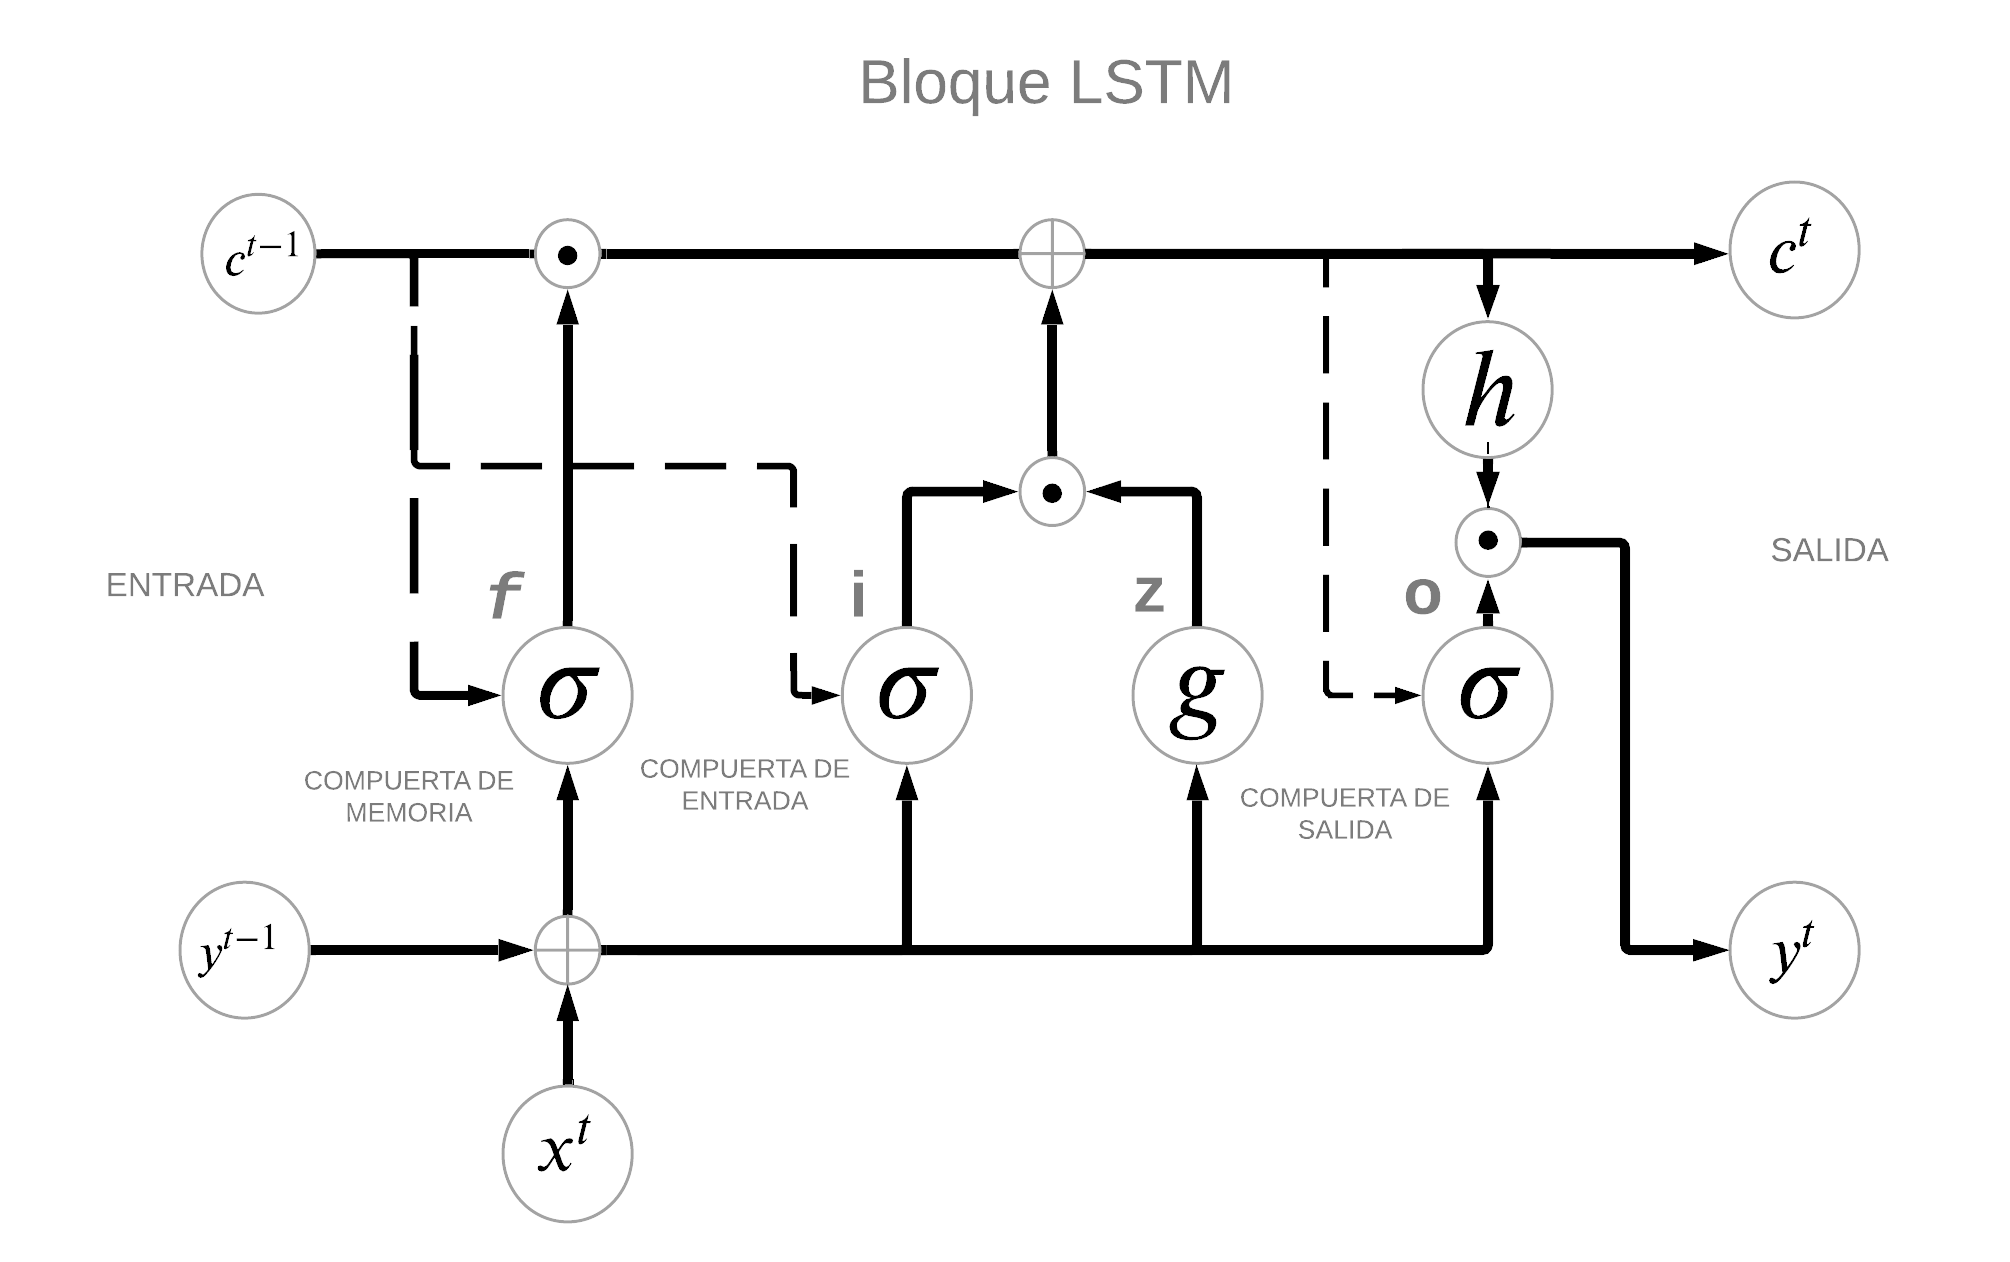
\includegraphics[width=0.5\textwidth]{imgs/diagrama-lstm.png}
    \caption{Diagrama del bloque LSTM.}
    \label{fig:diagrama-LSTM}
\end{figure}

Actualmente, este tipo de redes son las más utilizadas para realizar reconocimiento de caracteres, pero cuentan con la desventaja de un alto costo computacional, lo que desaconsejable su uso en sistemas embebidos.

\subsection{Redes CNN}

La otra alternativa que se puede utilizar son las CNN, que mediante filtros bidimensionales y una serie de capas totalmente conectadas se predice el texto más probable.
Al no requerir almacenar información ni trabajar de forma recursiva, la implementación
de este tipo de redes se puede hacer en equipos con un hardware de menor potencia, menor tamaño y, por consiguiente, menor costo. La mayor desventaja es que la cantidad de caracteres debe estar previamente definido.

Las patentes argentinas han sufrido tres modificaciones a lo largo de los años, que se pueden ver en la Fig. \ref{fig:patentes-arg}. En la actualidad, se pueden encontrar vehículos con las patentes lanzadas en 1994 y 2015. Si se considera un séptimo carácter en las de 1994 como un guion bajo (\_), es posible utilizar una red neuronal del tipo CNN frente a una LSTM.
\begin{figure}[h]
    \centering
    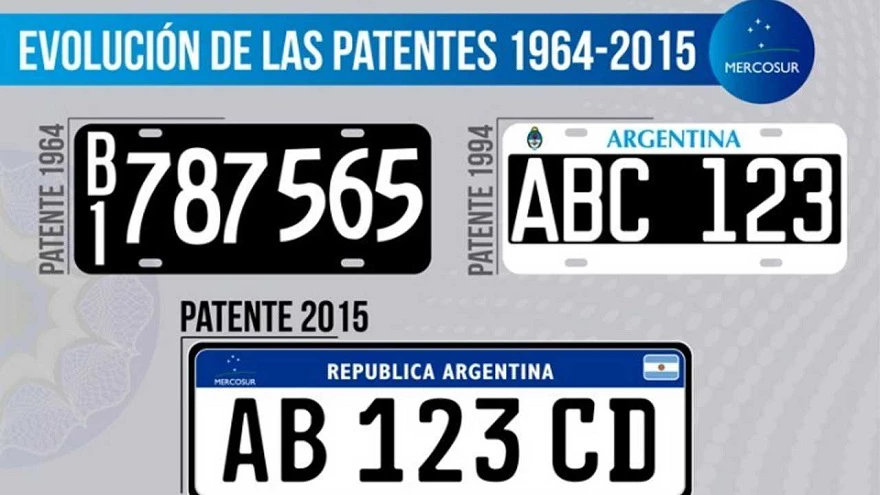
\includegraphics[width=0.5\textwidth]{imgs/patentes-arg.png}
    \caption{Evolución patentes Argentinas a lo largo de los años.}
    \label{fig:patentes-arg}
\end{figure}


\section{¿Qué es una red neuronal?}

Se entiende como red neuronal a un algoritmo computacional que intenta imitar el cerebro humano, en otras palabras, es un algoritmo de computación compuesto por un gran número de elementos simples que se
encuentran interconectados, los cuales procesan la información por medio de estados dinámicos, respondiendo a entradas externas, que permite realizar diversas tareas.
En este caso el trabajo se centrará en la tarea de clasificación de datos.
Debido a la semejanza que existe entre los algoritmos de Deep Learning \cite{ibm_que_nodate} (algoritmos de aprendizaje profundo) y el cerebro humano, a la unidad fundamental de estos sistemas se la denomina neurona.


\subsection{La neurona}

La neurona es la unidad fundamental dentro de la red, y su nombre viene de la similitud que existe entre este elemento y una neurona humana, esto se puede apreciar en Fig. \ref{fig:comparativa-neuronas}. La tarea de la neurona es procesar la información que le entra para producir un valor de salida, a este proceso se lo conoce como sinapsis.

\begin{figure}[h]
    \centering
    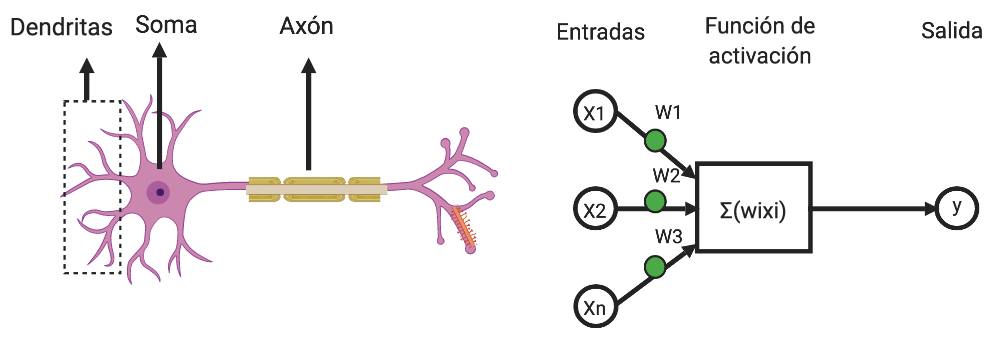
\includegraphics[width=1\textwidth]{imgs/comparacion-neurona-red.png}
    \caption{Comparación neurona con neurona artificial.}
    \label{fig:comparativa-neuronas}
    %https://futurelab.mx/redes%20neuronales/inteligencia%20artificial/2019/06/25/intro-a-redes-neuronales-pt-1/
\end{figure}

La sinapsis entre neuronas es una suma ponderada que puede ser expresada como $y =W^T \cdot X + b$ donde $y$ es el valor de salida de la neurona,
$W$ representa los pesos de la neurona y se define como un vector columna de dimensión $N$, $b$ es un bias y $X$ es el vector columna de dimensión $N$. Si bien la neurona es muy útil, sola no es de mucha utilidad, es por ello que a los arreglos en paralelo de neuronas se los denomina capa, a la conexión de capas de neuronas simples se las denomina capas totalmente conectadas, ya que toda la información de la capa anterior se envía a la capa siguiente.

\section{Redes neuronales}

A la hora de resolver problemas más complejos es usual necesitar más de una capa, es por ello que se interconectan para formar una red neuronal en la Fig. \ref{fig:esquema-redes} se observa una red con varias capas.

\begin{figure}[h]
    \centering
    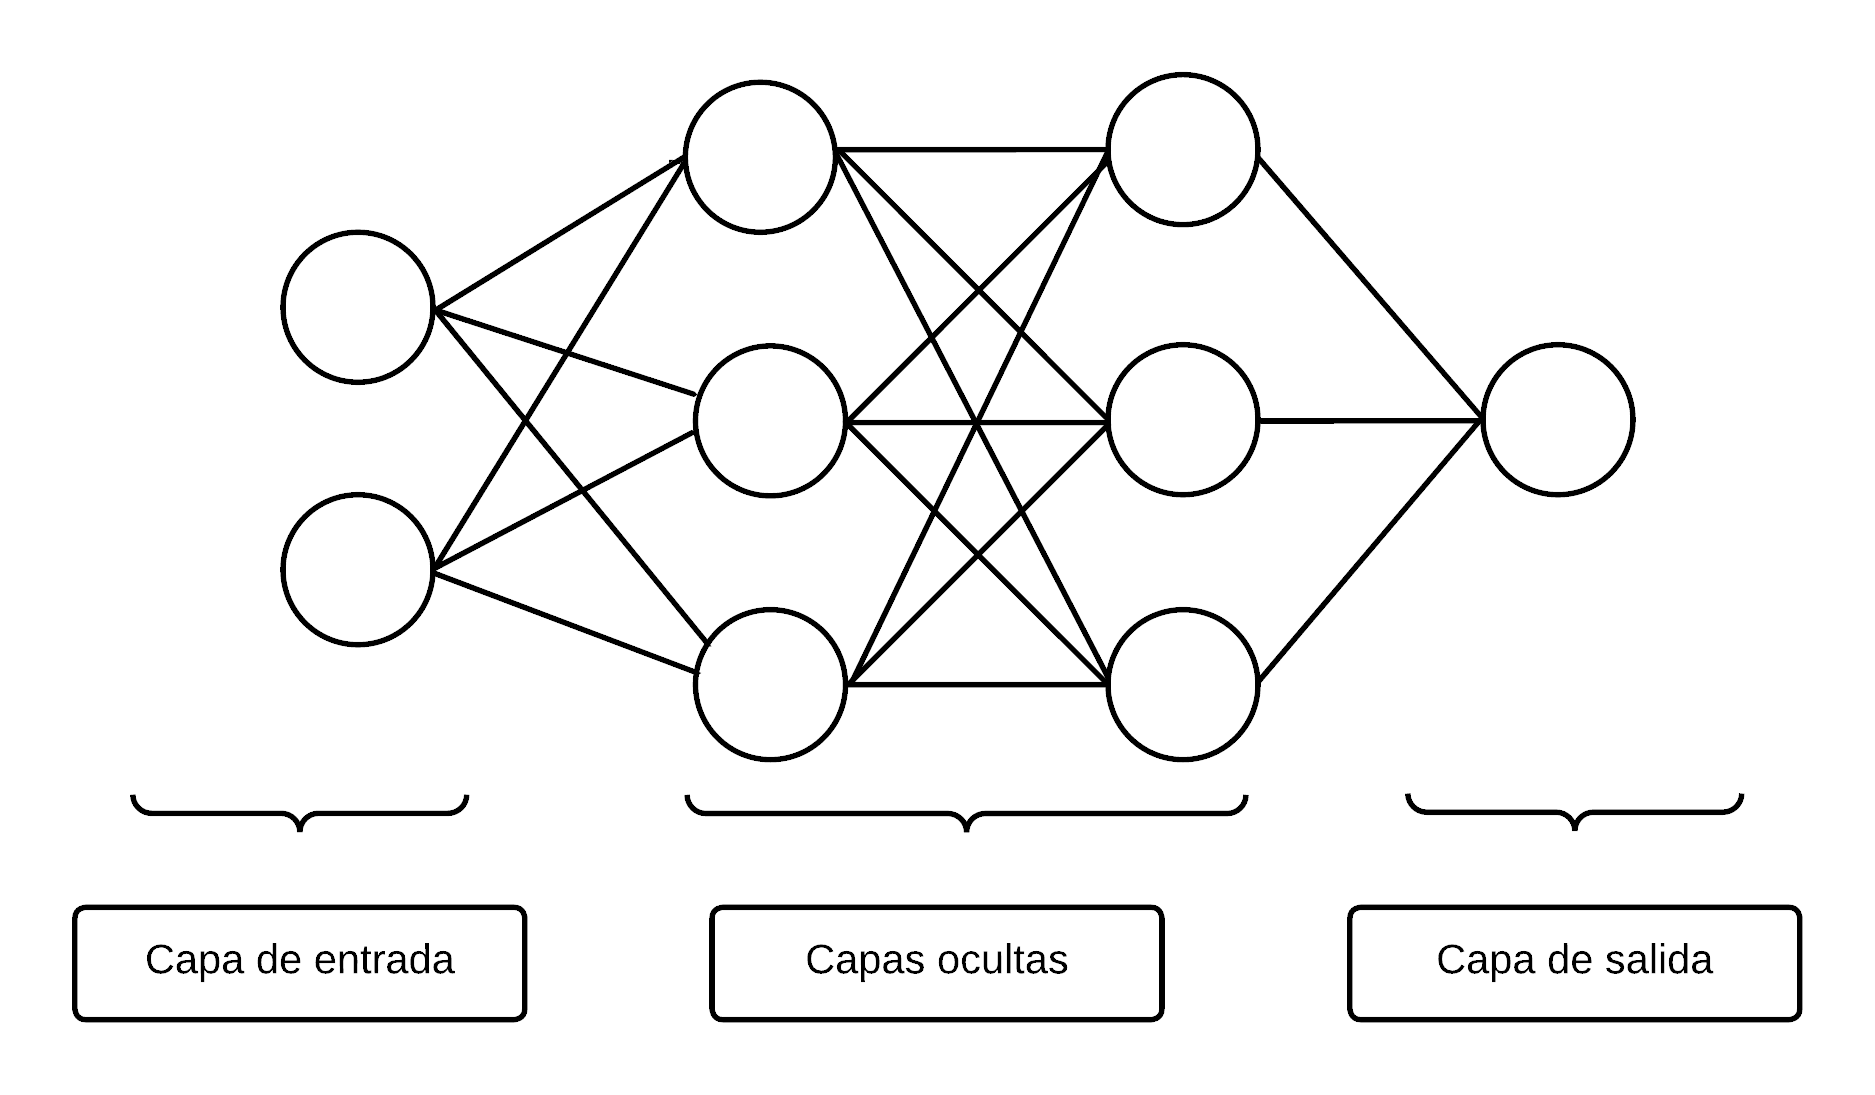
\includegraphics[width=0.6\textwidth]{imgs/Redes-esquema.png}
    \caption{Esquema simplificado de una red neuronal.}
    \label{fig:esquema-redes}
\end{figure}

Debido a que en esencia el proceso que realiza la neurona es una transformación lineal, al interconectar capas la resultante sigue siendo una transformación lineal.
Este problema de linealidad se soluciona aplicando una transformación no lineal, la cual se suele llamar función de activación,
luego de que la información es procesada por la neurona, obteniendo $y= f(W^T X + b)$. Las funciones de activación más conocidas se pueden observar en la Fig. \ref{fig:funciones-activacion}.

\begin{figure}
    \centering
    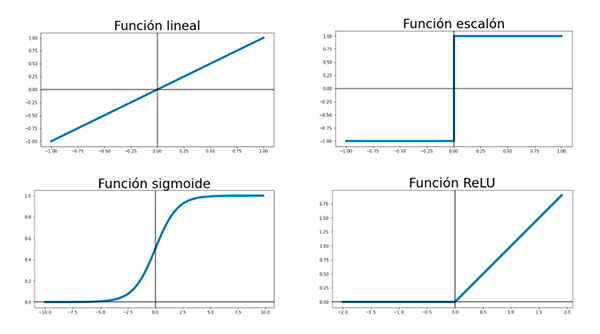
\includegraphics[width=1\textwidth]{imgs/Funciones-de-activacion.jpg}
    \caption{Funciones de activación más comunes.}
    \label{fig:funciones-activacion}
\end{figure}

En resumen una red funciona de la siguiente manera, se realiza la multiplicación de la entrada por los pesos de la red, luego los resultados son ingresados a la función de activación para quitar las linealidades. Posteriormente esta información se pasa a la capa siguiente y se realiza el mismo proceso. Esto se repite hasta llegar a la capa de salida donde, en tareas de clasificación, se suelen colocar tantas neuronas como salidas posibles.

\section{Redes neuronales de convolución}

Si bien, hasta ahora se han analizado solo las capas totalmente conectadas existen una gran cantidad de capas diferentes, para este trabajo se dará una breve introducción a las redes de convolución o CNN.

La función principal de las capas de convolución es poder extraer información de una imagen, es por ello que nace la semejanza entre las CNN y la corteza visual de los animales.
Este tipo de redes poseen características que las hacen únicas, por lo que se estudiarán las partes que la componen.
En la Fig. \ref{fig:esquema-CNN} se observa un esquema de la misma.
\begin{itemize}
    \item Capa convolucional: capa principal de las CNN, sus parámetros son básicamente filtros entrenables de dimensiones determinadas por el
          usuario, que realiza una multiplicación punto a punto recorriendo toda la imagen y produciendo un mapa de activación bidimensional, es decir, otra imagen. En la
          Fig. \ref{fig:esquema-capa-convolucional} se ve el funcionamiento de esta capa. Cada uno de los filtros se activarán según la característica que aprenda la red.
    \item Capa de agrupación: se coloca entre las capas de convolución, toma los mapas de características producidos por la capa de
          convolución y los agrupa en una imagen. En esta capa se produce una reducción de la dimensión, lo que reduce la complejidad para evitar el sobreajuste de los parámetros.
    \item Función de activación.
    \item Capa de aplanamiento o Flatten: Antes de pasar las salidas de las capas convolucionales se produce un aplanamiento de las imágenes, esta capa transforma las imágenes o matrices de dimensión $N \times N$ en un vector columna $2NM$, donde $M$ es la cantidad de filtros de la capa anterior.
    \item Capa completamente conectada: Se encargan de procesar la información de los filtros para obtener la cantidad de salidas esperadas.
\end{itemize}

Si bien la descripción de las capas de convolución, agrupación y función de activación se realizaron de forma separa, se suelen implementar juntas, ya que es común tener varias capas de convolución conectadas en serie, permitiendo extraer información más especifica de la red.

\begin{figure}
    \centering
    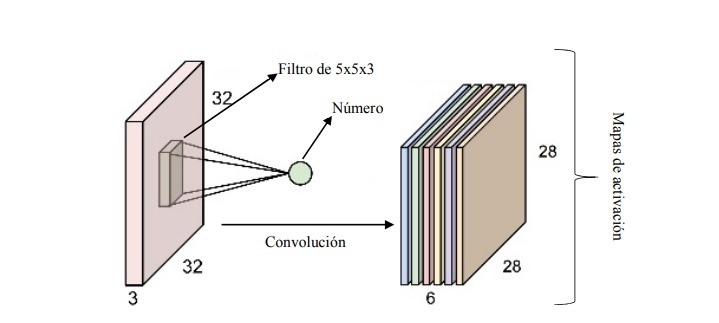
\includegraphics[width=1\textwidth]{imgs/capa-convolucional.jpeg}
    \caption{Esquema de funcionamiento de una capa convolucional.}
    \label{fig:esquema-capa-convolucional}
\end{figure}
\begin{figure}
    \centering
    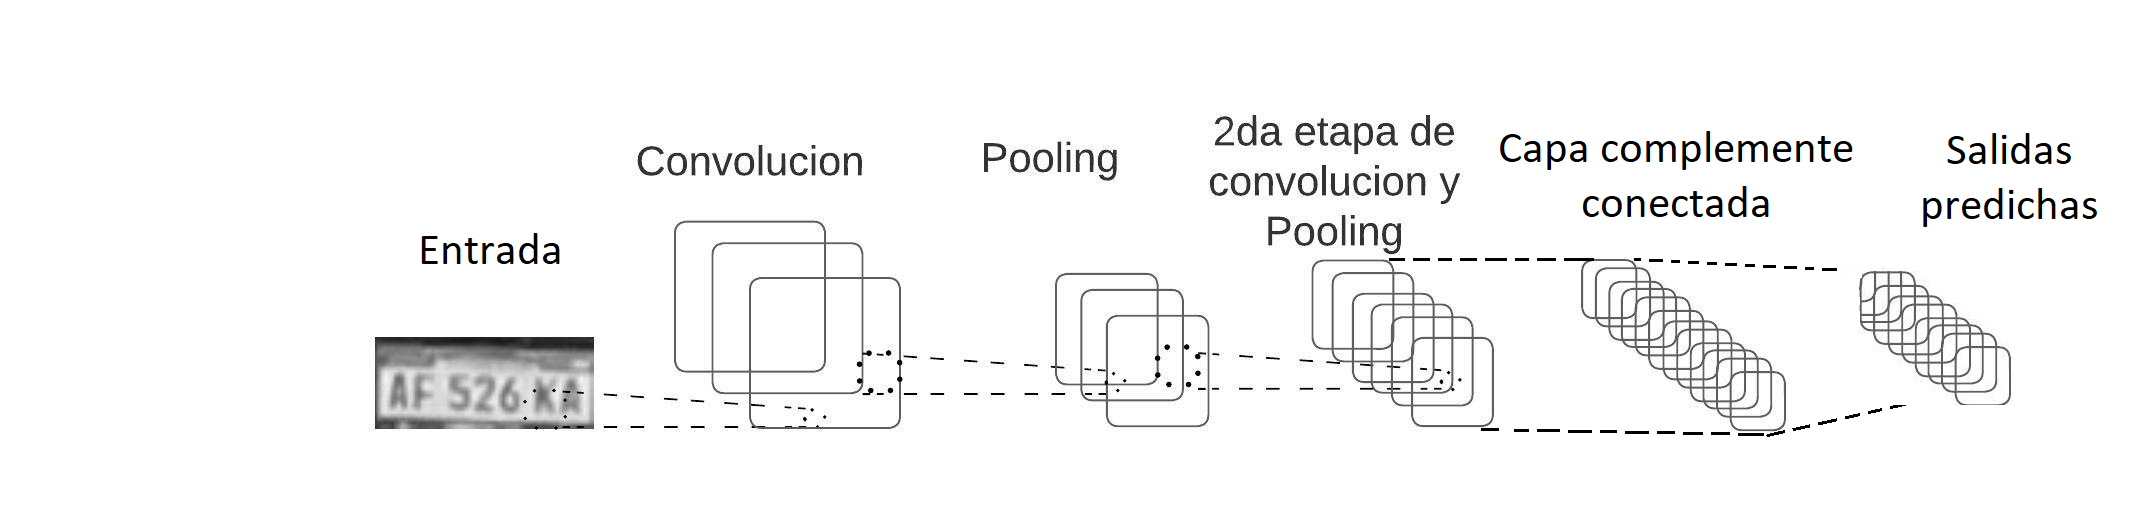
\includegraphics[width=1\textwidth]{imgs/CNN-completa.png}
    \caption{Ejemplificación de una red neuronal de convolución.}
    \label{fig:esquema-CNN}
\end{figure}

\subsection{Convolución en 2D}

La convolución bidimensional es similar al caso conocido en 1D, pero en este caso se desplaza una submatriz de un tamaño predefinido, comúnmente denominado kernel, por la matriz o imagen de entrada.

Se define kernel a la respuesta de un sistema discreto, el cual es de dimensión $2k \times 2k$, donde $k$ es un
valor establecido arbitrario (usualmente se utilizan matrices de $3 \times 3$ o $5 \times 5$) que define cuántos valores de la muestra habrá.

Se define a $h[n,m]$ como un filtro de dimensión $(2k + 1) \times (2k + 1)$ e $I$ una imagen a escala de grises, donde cada punto de coordenadas $(i,j)$ es el
resultado de la convolución entre $h$ e $I$ dado por

\begin{equation}
    O(i,j)= \sum_{u=-k}^{k} \sum_{v=-k}^{k} h[u,v]I[i-u,j-v]
\end{equation}

Esta operación consiste en filtrar una subimagen de dimensión $(2k+1)\times(2k+1)$ en la imagen $I$ original para cada pixel centrado en dicha imagen, calculando la operación de convolución y dando como resultado un pixel de la imagen de salida $O$.
este proceso
\subsection{Capa de agrupación}

La capa de agrupación o pooling se encarga de reducir el tamaño de la imagen ejecutando una función a una submatriz de $n \times n$ de la imagen pasando de tener $n^2$ elementos a un elemento, las funciones de polling más utilizadas son:

\begin{itemize}
    \item MaxPooling: se queda con el valor máximo de la submatriz.
    \item AveragePooling: calcula la media de los elementos.
\end{itemize}

Otra forma de entender a la capa de pooling es un submuestreo de la imagen de salida de la capa de convolución que devuelve el valor más significativo.

En la Fig. \ref{fig:ejemplo-mp} se puede apreciar el comportamiento de una capa de maxpooling. Luego de la capa de convolución, se divide la matriz
en pequeñas matrices de $2 \times 2$ y se extrae el valor más representativo de cada submatriz, reduciendo la matriz de un tamaño de $5 \times 5$ a una de $3 \times 3$, en este caso.
\begin{figure}
    \centering
    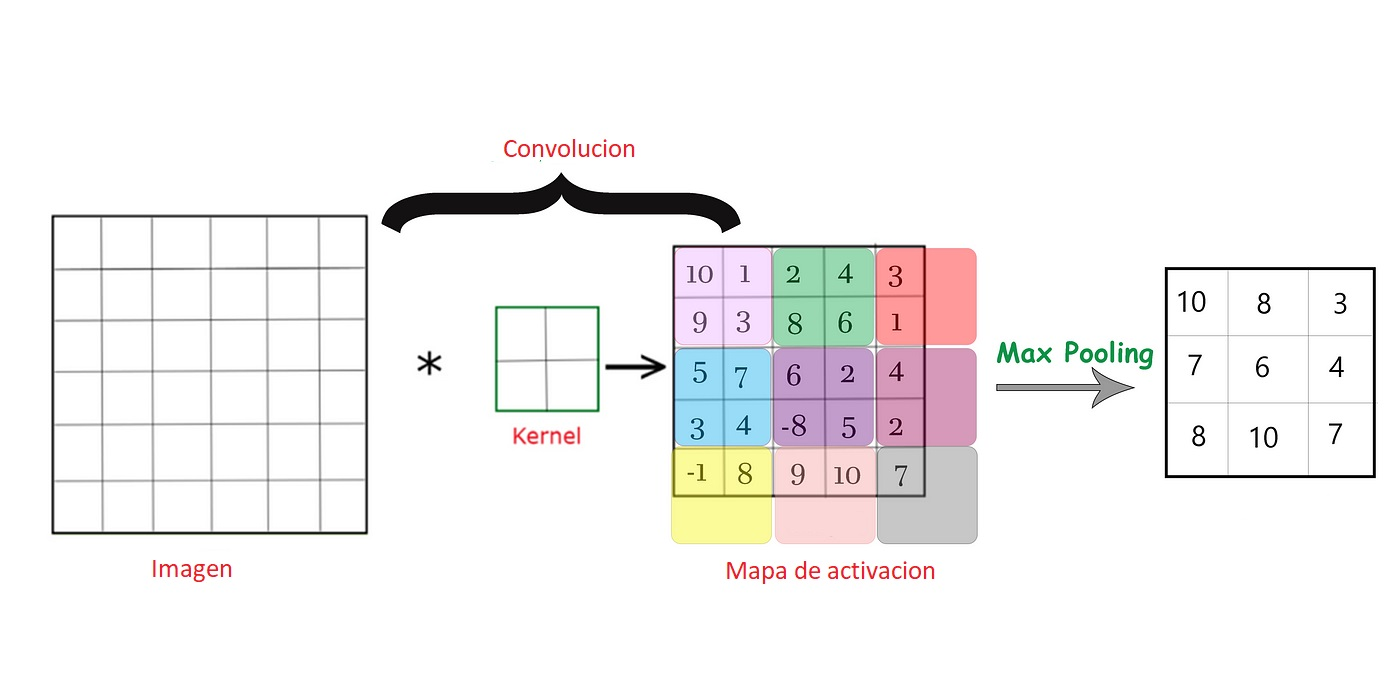
\includegraphics[width=1\textwidth]{imgs/ej-maxpooling.jpg}
    \caption{Ejemplo de funcionamiento de Maxpooling.}
    \label{fig:ejemplo-mp}
\end{figure}

\subsection{Técnica de Batch-Normalization}

La técnica de Batch-Normalization se utiliza para reducir la covarianza de los datos de entrada. Esto se realiza normalizando los datos de entrada en un rango de 0 a 1 evitando trabajar con números grandes. Si bien este proceso se suele realizar con los datos de entrada, es útil realizarlo entre capas antes de la función de activación para trabajar siempre con datos normalizados, lo que permite un ajuste de parámetros más simple. Finalmente antes de pasar a la capa siguiente se aplica la función de activación.

\section{CCN-OCR}

Para este trabajo se utilizó una CNN diseñada y entrenada por Ankadrew, cuya arquitectura se puede ver en Fig. \ref{fig:arquitectura-cnn-ocr}. De la arquitectura de la red se destaca la capa de Global Average Pooling, la cual remplaza a la capa de aplanamiento y calcula la media por cada imagen de salida de la capa anterior, produciendo un valor por cada imagen [incluir figura de la diferencia de una capa de Flatten y un global average pooling].
\begin{figure}
    \centering
    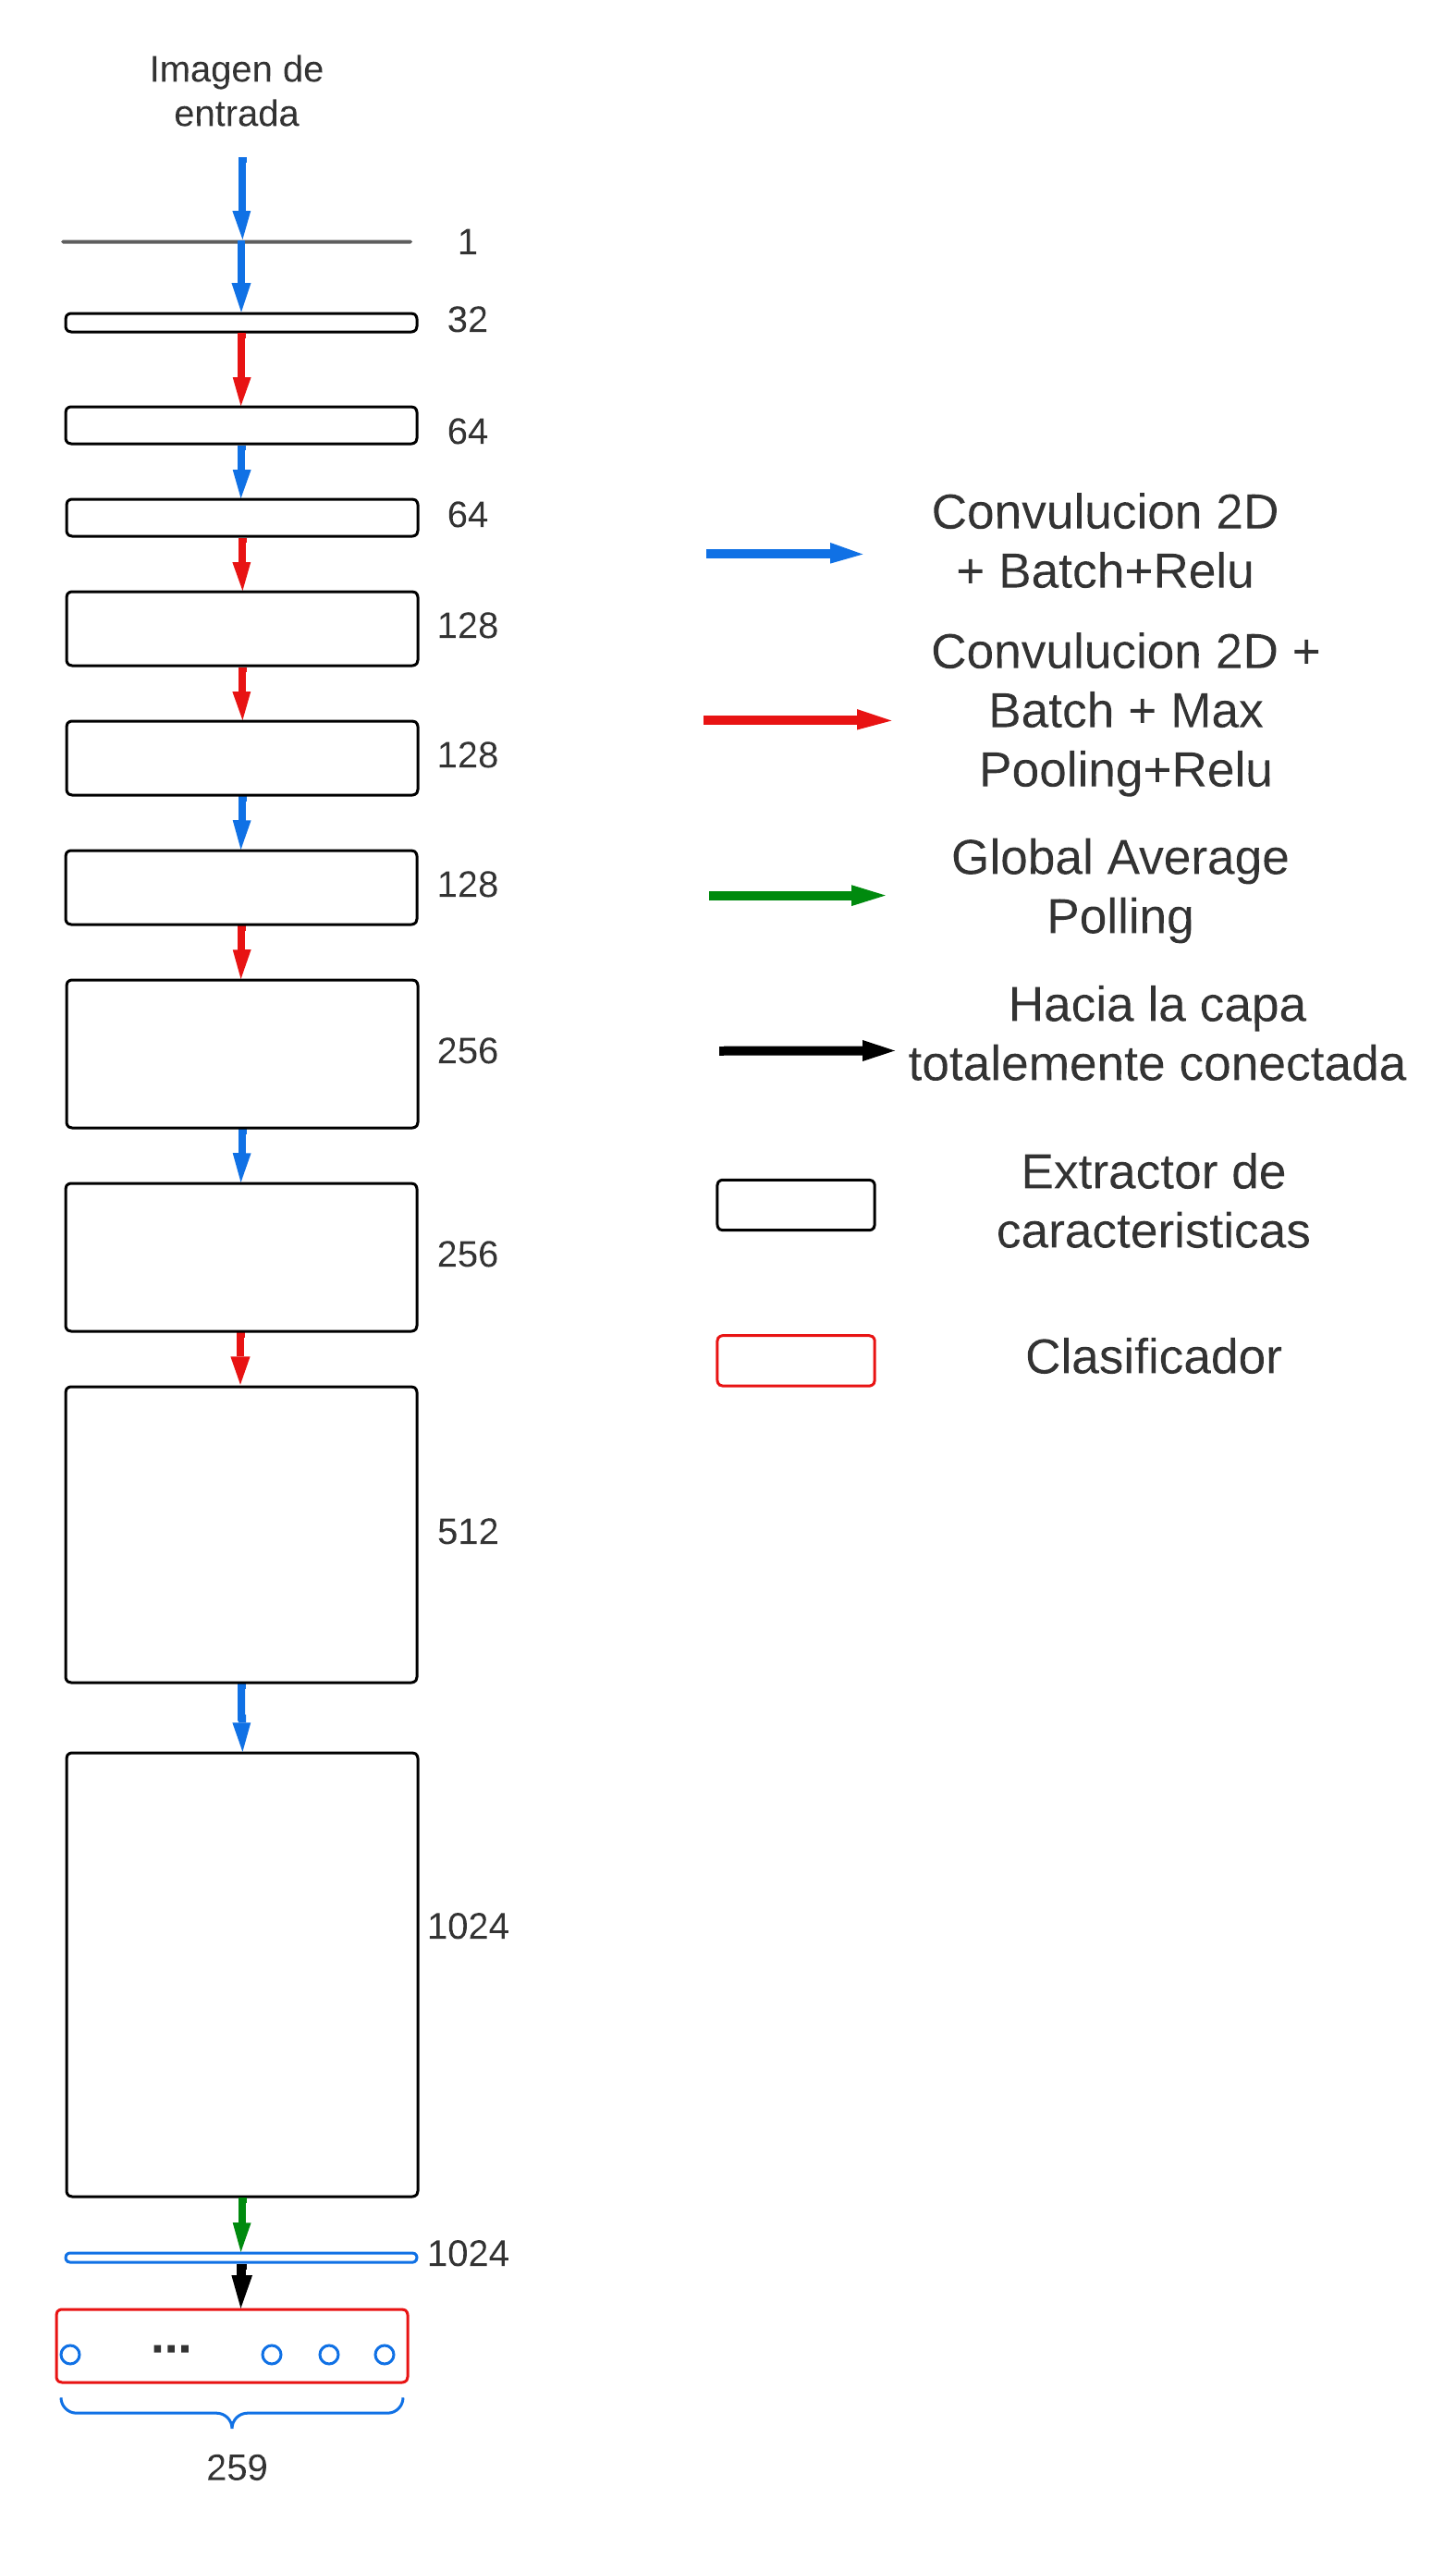
\includegraphics[width=.4\textwidth]{imgs/cnn-ocr.png}
    \caption{Arquitectura de la CNN-OCR.}
    \label{fig:arquitectura-cnn-ocr}
\end{figure}

Otro elemento a destacar de la red son las siete capas densas conectadas en paralelo, debido a que, como se anticipó en secciones anteriores, las patentes poseen siete caracteres. En esencia cada capa densa es idéntica, solo se diferencian sus pesos que son aprendidos durante el entrenamiento de la misma. Cada capa posee en total treinta y siete caracteres de salida, esto surge de las veintiseis letras del abecedario, los diez números del 0 al 9 y el símbolo de guion bajo (\_) utilizado en el caso de las patentes antiguas que solo poseen seis caracteres.

Como aclaración para el resto del trabajo, se referirá a esta red como CNN-OCR.

\subsection{Requerimientos}

Si bien la CNN es muy útil para la tarea a resolver, posee una serie de requisitos previos en la imagen de entrada. Según el autor, la CNN
necesita como entrada una imagen de la patente en blanco y negro de dimensiones $70 \times 140$ pixeles.
Por lo que es necesario realizarle un tratamiento previo a las imágenes antes de ingresarlas por la CNN-OCR. El tratamiento necesario
se puede observar en la Fig. \ref{fig:Comparativa-imagenes}. Entonces existen tres pasos previos luego de sacar
la captura antes de ingresarla a la CNN-OCR:

\begin{enumerate}
    \item Obtener un recorte de la patente.
    \item Transformar la imagen a escala de grises.
    \item Redimensionar la imagen al tamaño requerido.
\end{enumerate}
\begin{figure}
    \centering
    \begin{subfigure}[b]{0.49\textwidth}
        \centering
        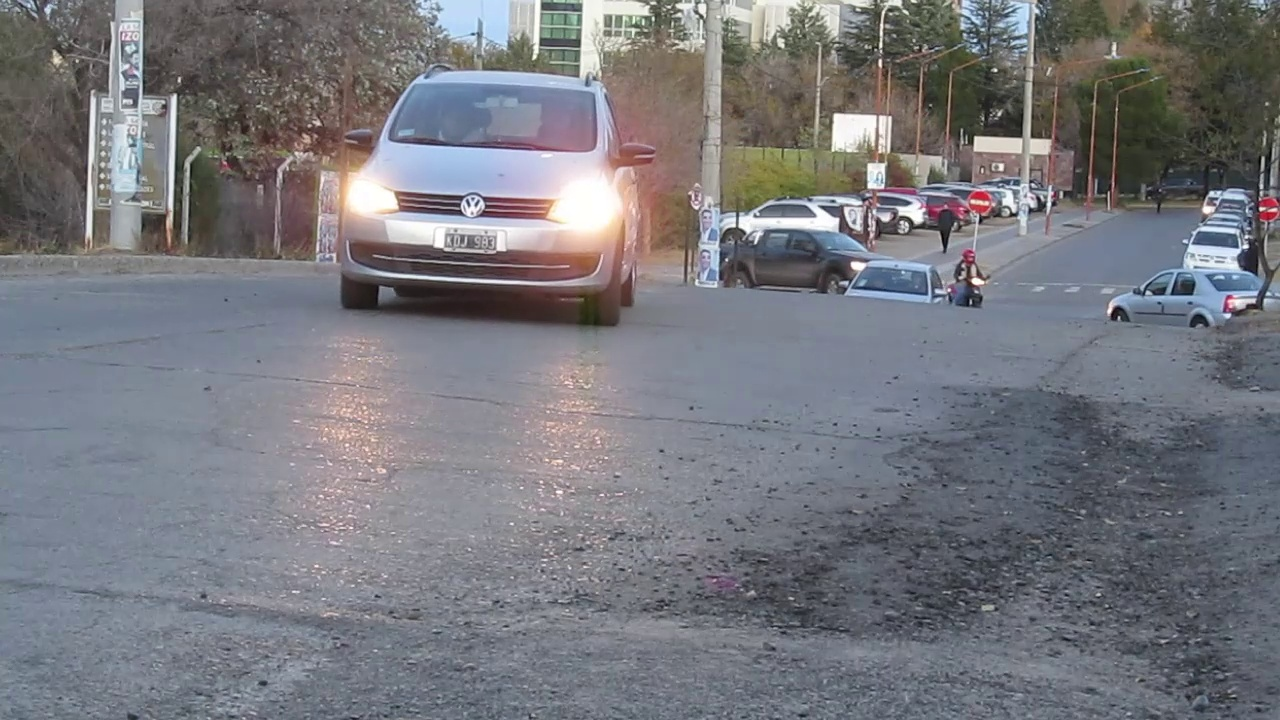
\includegraphics[width=\textwidth]{imgs/imagen-obtenida.jpg}
        \caption{Imagen obtenida por la cámara.}
        \label{fig:imagen-obtenida}
    \end{subfigure}
    \hfill
    \begin{subfigure}[b]{0.49\textwidth}
        \centering
        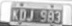
\includegraphics[width=0.7\textwidth]{imgs/imagen-requerida.jpg}
        \caption{Imagen requerida por la CNN-OCR.}
        \label{fig:imagen-requerida}
    \end{subfigure}
    \caption{Ejemplo de imagen obtenida e imagen requerida por la CNN-OCR.}
    \label{fig:Comparativa-imagenes}
\end{figure}

\subsubsection*{Obtención del recorte de la patente}

Debido a la importancia de esta etapa y a su complejidad, se realiza una explicación extendida, con la finalidad de tener una mejor comprensión del funcionamiento del proceso de recorte necesario para que la CNN-OCR pueda funcionar de manera óptima. Siguiendo la recomendación del autor de CNN-OCR, se utilizó una red complementaria que detecta la ubicación de la patente y luego realiza el recorte. La red recomendada para esta tarea es la Yolo (You Only Look Once) en su versión 4 o YoloV4 \cite{bochkovskiy_yolov4_2020}.

El modelo de la YoloV4 es un sistema de código abierto el cual se centra en la detección de objetos. Utiliza una arquitectura Darknet \cite{noauthor_darknet_nodate}, escrita en C, que se puede ver en la Fig.\ref{fig:funcionamiento-yolo}.
Una de las principales características de esta arquitectura es la forma en que realiza el proceso de detección y posterior clasificación. La red se puede entender como tres partes diferentes que, para mantener la nomenclatura de la propia arquitectura, no fueron traducidas y se mantendrán en inglés. Estas partes son:

\begin{itemize}
    \item Head: es la parte encargada de reconocer objetos, básicamente busca una región en la que pueda haber un objeto, sin distinguir cuál sea. Se utilizan dos etapas de detectores, la primera utiliza subimágenes de tamaño fijo, y la otra varía el tamaño de las subimágenes para adecuarse mejor al tamaño de cada objeto.
    \item Backbone: es una arquitectura de deep learning que actúa como extractor de características. Es, en esencia, un modelo de clasificación. Se encarga de tomar las ubicaciones obtenidas por el Head y clasificar sí son o no los objetos requeridos. Es la única parte de la red que se modifica y entrena dependiendo el entorno en que se desea utilizar.
          En el caso de este trabajo el Backbone fue entrenado por el mismo autor de la CNN-OCR para que reconozca patentes argentinas \cite{ankandrew_localizador_2021}.
    \item Neck: su funcionalidad es tomar mapas de característica de diferentes partes del Backbone y agregarle características, para facilitar la clasificación de los objetos.
\end{itemize}

Debido a que la Darknet está escrita en C es necesario compilar la misma, esto se hizo siguiendo los pasos del repositorio de AlexeyAB \cite{alexey_yolo_2023}.


\begin{figure}
    \centering
    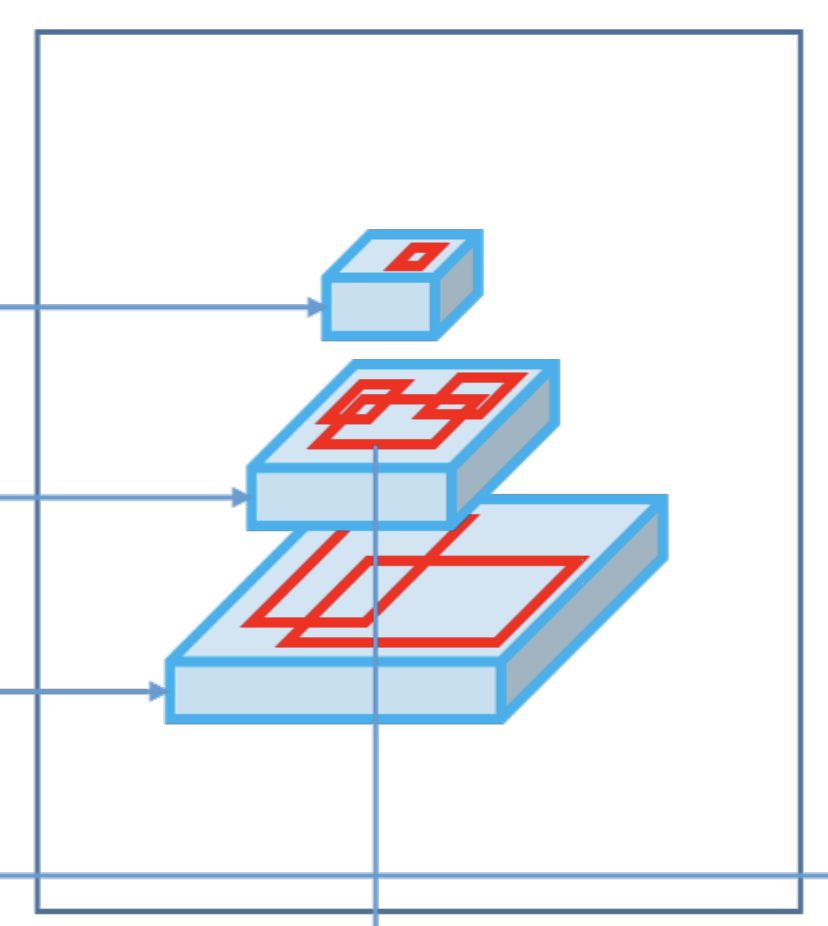
\includegraphics[width=0.5\textwidth]{imgs/funcionamiento-yolo.png}
    \caption{Funcionamiento del proceso de detección de la YoloV4 \cite{bochkovskiy_yolov4_2020}.}
    \label{fig:funcionamiento-yolo}
\end{figure}

\subsubsection*{Transformación a escala de grises}

El proceso de conversión a escala de grises se puede hacer de diversas maneras. La forma más utilizada es realizar un promedio de las capas de color Rojo ($R$), Verde ($G$), Azul ($B$) quedando descripto por la eq. \ref{eq:gray-mean}. Existe otra forma utilizando un promedio ponderado para compensar la sensibilidad relativa del ojo humano la cual se puede observar en la eq. \ref{eq:gray-human}. En la Fig. \ref{fig:comparacion-grises} se observa que el método de escala de grises teniendo en cuenta la sensibilidad del ojo humano obtiene un mejor resultado.

\begin{equation}
    \label{eq:gray-mean}
    I = \frac{R + G + B}{3}
\end{equation}

\begin{equation}
    \label{eq:gray-human}
    I = 0.2989R + 0.587G + 0.114B
\end{equation}

\begin{figure}
    \centering
    \begin{subfigure}[b]{0.3\textwidth}
        \centering
        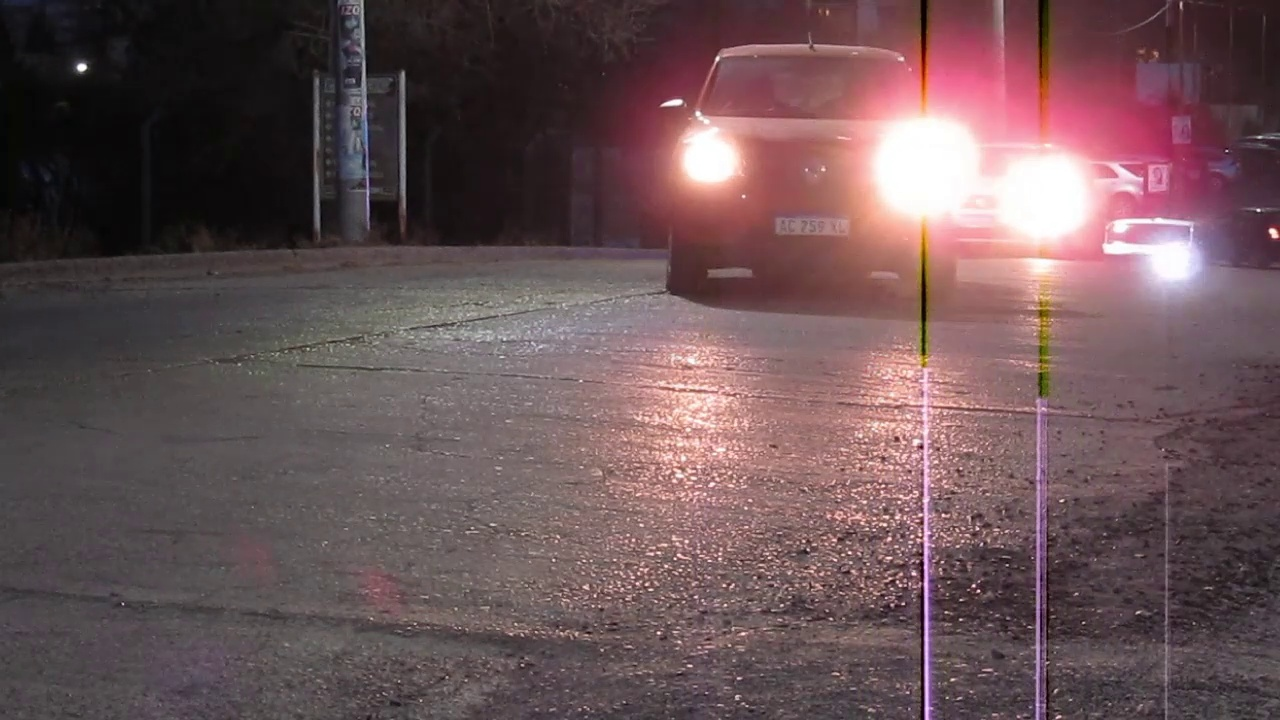
\includegraphics[width=\textwidth]{imgs/escala-grises-original.jpg}
        \caption{Imagen original.}
    \end{subfigure}
    \hfill
    \begin{subfigure}[b]{.3\textwidth}
        \centering
        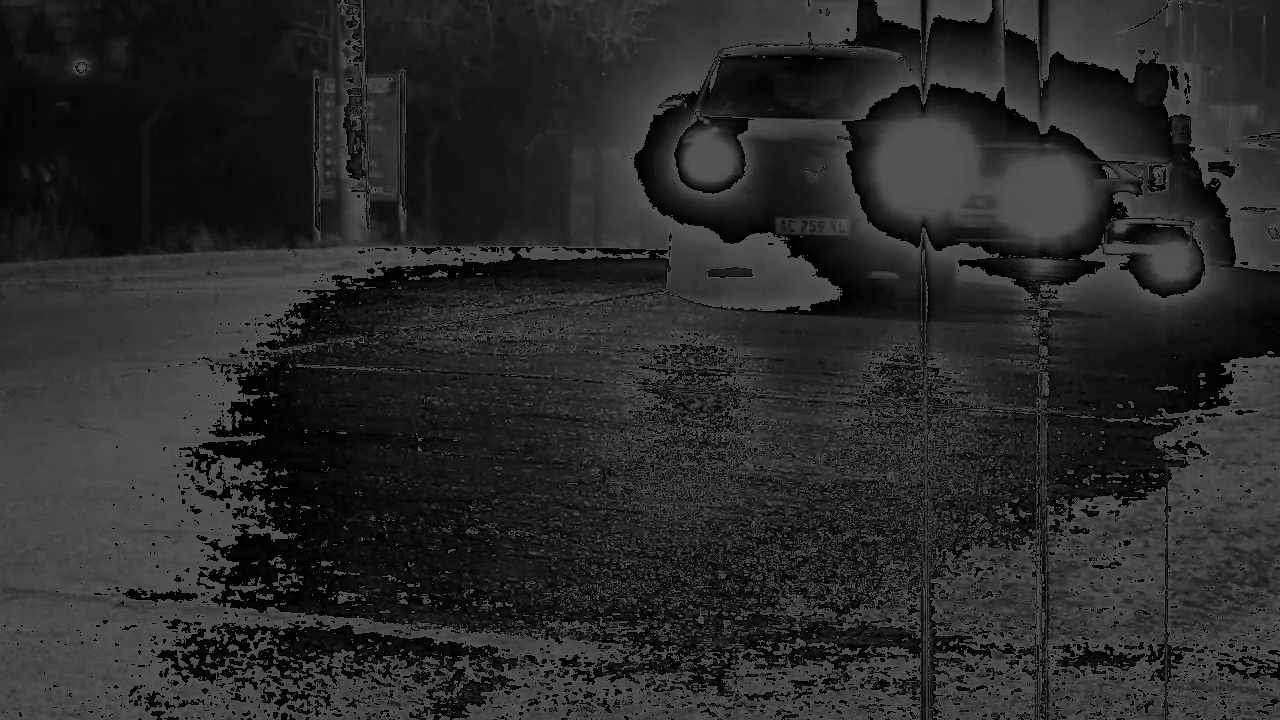
\includegraphics[width=\textwidth]{imgs/escala-grises-promedio.jpg}
        \caption{Promedio.}
    \end{subfigure}
    \hfill
    \begin{subfigure}[b]{.3\textwidth}
        \centering
        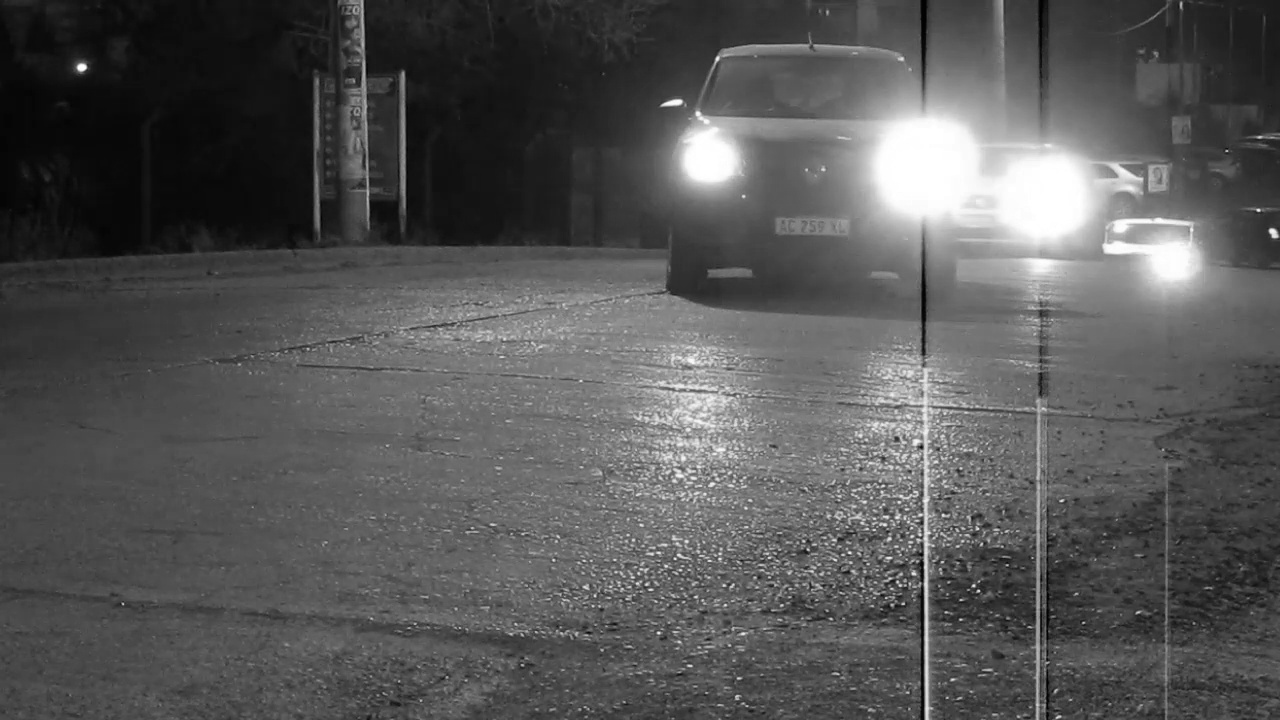
\includegraphics[width=\textwidth]{imgs/escala-grises-sensibilidad.jpg}
        \caption{Promedio ponderado.}
    \end{subfigure}
    \hfill
    \caption{En a) se observa la imagen original, mientras que en b) y c) la imagen convertida a escala de grises por los diferentes métodos.}
    \label{fig:comparacion-grises}
\end{figure}

\subsubsection*{Redimensionamiento de la imagen}

Para redimensionar la imagen se utiliza una interpolación bilineal la cual no se explicará en este trabajo debido a la complejidad del algoritmo.

\section{Implementación del algoritmo en Python 3}

Para la implementación del algoritmo se utilizó el lenguaje Python 3, ya que cuenta con una gran cantidad de librerías necesarias para el funcionamiento del sistema completo. La descripción general del algoritmo se puede observar en Fig. \ref{fig:algoritmo-ocr}.

\begin{figure}
    \centering
    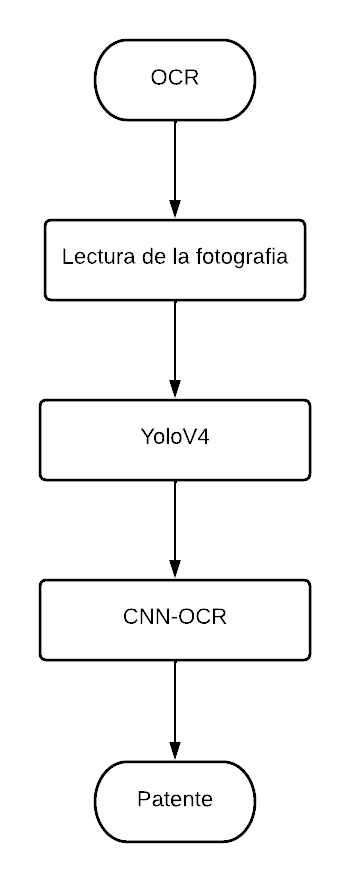
\includegraphics[width=.25\textwidth]{imgs/flujo-algoritmo-ocr.png}
    \caption{Algoritmo general de OCR.}
    \label{fig:algoritmo-ocr}
\end{figure}


\begin{figure}[h]
    \centering
    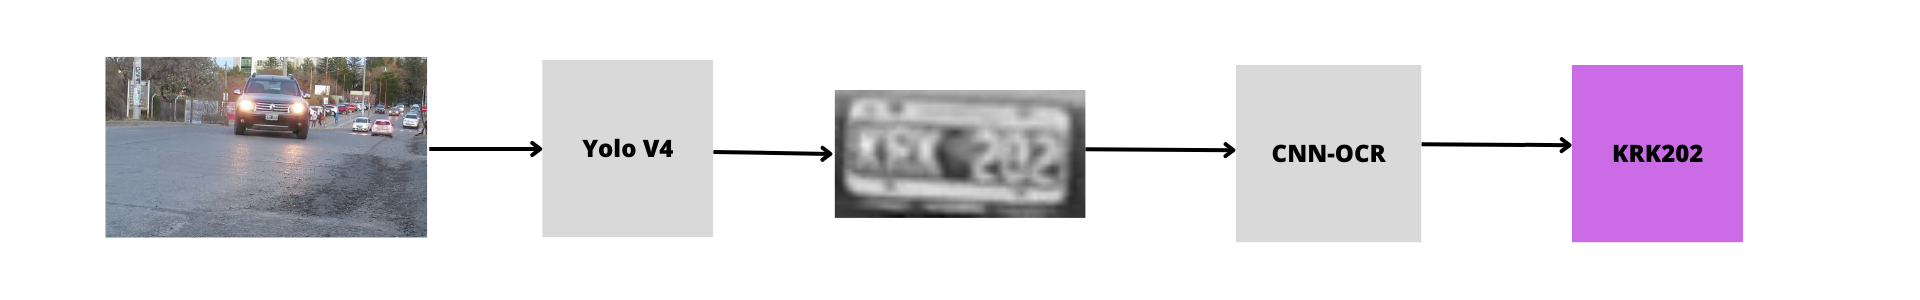
\includegraphics[width=\textwidth]{imgs/pic-to-text.png}
    \caption{Flujo de una fotografía hasta obtener el texto de la patente.}
    \label{fig:pic-to-text}
\end{figure}


La lectura u obtención de una fotografía se realizó mediante OpenCV \cite{opencv_opencv_2023} ya que permite utilizar una gran variedad de fuentes tales como cámaras y archivos. Luego se procesa mediante la YoloV4, que devuelve la ubicación relativa de la patente en la imagen en un archivo de texto plano para, posteriormente, leer el archivo de texto, junto con las dimensiones de la imagen y poder obtener la patente recortada. Antes de pasar el recorte a la CNN-OCR se la cambia a escala de grises y se la lleva al tamaño de $70 \times 140$ utilizando una interpolación lineal y se normalizan los valores de la imagen entre 0 y 1 usando OpenCV. Finalmente se procesa la imagen por la CNN-OCR obteniendo la patente en texto. En capítulos posteriores se explicará en mayor detalle que sucede con la imagen, y la patente obtenida (Fig. \ref{fig:pic-to-text}).


\subsection{Prueba de rendimiento}

Con la finalidad de dimensionar los tiempos de procesamiento del algoritmo de OCR, se procesaron diez imágenes y luego, se calculó el promedio para obtener el tiempo promedio por imagen en diferentes sistemas. Los resultados se encuentran en Tab. \ref{tab:ocr}.
Luego de analizar los tiempos obtenidos, se observa que la Raspberry Pi tarda demasiado en procesar una imagen, mientras que los otros sistemas poseen tiempos similares.
\begin{table}
    \centering
    \begin{tabular}{ccccc}
        \toprule
                   & Raspberry Pi 3b+ & Jetson TX1 & I5-11600K & I5-1135G7 \\
        \midrule
        Tiempo [s] & 85.78            & 6.15       & 1.05      & 1.20      \\
        \bottomrule
    \end{tabular}
    \caption{Tiempos obtenidos del procesamiento de diez imágenes.}
    \label{tab:ocr}
\end{table}



